\documentclass[british]{ntnuthesis}

% \title{Interpretable Machine Learning Models for DAS Data}
\title{Parallel Processing and Anomaly Detection of DAS Data using Autoencoders: Enhancing Efficiency in Large-Scale Sensor Data Analysis}
\shorttitle{Parallel Processing and Anomaly Detection on DAS data}
\author{Jørgen Aleksander Fagervik \\
        Supervisor: Ole Jakob Mengshoel}
\shortauthor{J. A. Fagervik}
\date{CC-BY \ntnuthesisdate}

\addbibresource{thesis.bib}


% From https://www.overleaf.com/learn/latex/Glossaries

\makeglossaries % Prepare for adding glossary entries

\newglossaryentry{julia}
{
        name=Julia,
        description={Is an all-purpose programming language specially suited for
scientific computing}
}

\newglossaryentry{python}
{
        name=Python,
        description={Is an all-purpose general programming language suited for scripting, data-science and web applications}
}

\newglossaryentry{llvm}
{
        name=LLVM,
        description={Low Level Virtual Machine, better known as LLVM, is a project trying to provide a modern, SSA-based compilation strategy capable of supporting both static and dynamic compilation of arbitrary programming languages \cite{llvm}}
}

\newglossaryentry{fftw}
{
        name=FFTW,
        description={Fastest Fourier Transform in the West is one of the most famous implementations of the \acrshort{dft} algorithm. It is specialized for running on \acrlong{cpu}s}
}

\newglossaryentry{relu}
{
    name=ReLU,
    description={Rectified Linear Unit is one of the most commonly used activation functions within \acrshort{dnn}s}
}

\newglossaryentry{bibliography}
{
        name=bibliography,
        plural=bibliographies,
        description={A list of the books referred to in a scholarly work,
typically printed as an appendix}
}

\newglossaryentry{maths}
{
    name=mathematics,
    description={Mathematics is what mathematicians do}
}
\newglossaryentry{pubdas}
{
    name=PubDAS,
    description={A PUBlic Distributed Acoustic Sensing Datasets Repository for Geosciences}
}

\newglossaryentry{idun}{
    name=IDUN,
    description={The Idun cluster is a project between NTNU's faculties and the IT division that aims at providing a high-availability and professionally administrated compute platform for NTNU}
}

\newglossaryentry{svm}
{
    name=Support Vector Machine,
    description={Common machine learning technique}
}




% --------------------
% ----- Acronyms -----
% --------------------

\newacronym{ntnu}{NTNU}{Norwegian University of Science and Technology}
\newacronym{ai}{AI}{Artificial Intelligence}
\newacronym{ast}{AST}{Abstract Syntax Tree}
\newacronym{mb}{MB}{Megabyte}
\newacronym{gb}{GB}{Gigabyte}
\newacronym{tb}{TB}{Terrabyte}
\newacronym{ml}{ML}{machine learning}
\newacronym{fft}{FFT}{Fast Fourier Transform}
\newacronym{rfft}{RFFT}{Fast Fourier Transform for Real Numbers}
\newacronym{dft}{DFT}{Discrete Fourier Transform}
\newacronym{mpi}{MPI}{Message-passing interface}
\newacronym{ram}{RAM}{Random-access memory}
\newacronym{gcd}{GCD}{Greatest Common Divisor}
\newacronym{hpc}{HPC}{High Performance Computing}
\newacronym{api}{API}{Application program interface}
\newacronym{gpu}{GPU}{Graphics processing unit}
\newacronym{tpu}{TPU}{Tensor processing unit}
\newacronym{cpu}{CPU}{Central processing unit}
\newacronym{das}{DAS}{Distributed acoustic sensing}
\newacronym{ann}{ANN}{Artificial neural network}
\newacronym{cnn}{CNN}{Convolutional neural network}
\newacronym{rnn}{RNN}{Recurrent Neural Network}
\newacronym{dnn}{DNN}{Deep Neural Network}
\newacronym{repl}{REPL}{Read-eval-print loop}
\newacronym{lstm}{LSTM}{Long short-term memory}
\newacronym{jit}{JIT}{Just-in-time}
\newacronym{hdf}{HDF}{Hierarchical Data Format}
\newacronym{hdf5}{HDF5}{Hierarchical Data Format version 5}
\newacronym{sisd}{SISD}{Hierarchical Data Format version 5}
\newacronym{simd}{SIMD}{Single instruction, multiple device}
\newacronym{misd}{MISD}{Multiple instructions, single device}
\newacronym{mimd}{MIMD}{Multiple instructions, multiple device}
\newacronym{spmd}{SPMD}{Single program, multiple device}
\newacronym{cgf}{NTNU CGF}{NTNU Centre for Geophysical Forecasting}
\newacronym{posix}{POSIX}{Portable Operating System Interface}
\newacronym{asn}{ASN}{ALCATEL SUBMARINE NETWORKS}
\newacronym{dsp}{DSP}{Digital Signal Processing}
\newacronym{adam}{ADAM}{Adaptive Moment estimation}
\newacronym{sgd}{SGD}{Stochastic Gradient Descent}
\newacronym{gru}{GRU}{Gated Recurrent Unit}
\newacronym{llm}{LLM}{Large Language Model}
\newacronym{sota}{SOTA}{State of the Art}
\newacronym{dl}{DL}{Deep Learning}
\newacronym{vae}{VAE}{Variational Autoencoder}
\newacronym{mae}{MAE}{Mean Absolute Error}
\newacronym{mse}{MSE}{Mean Squared Error}
\newacronym{gan}{GAN}{Generative Adverserial Network}
\newacronym{dbscan}{DBSCAN}{Density-Based Spatial Clustering of Applications with Noise}
\newacronym{adagrad}{AdaGrad}{Adaptive Gradient Algorithm}
\newacronym{fir}{FIR}{Finite Impulse Response}
\newacronym{elbo}{ELBO}{Evidence Lower BOund}
\newacronym{roi}{ROI}{Range of Interest}
\newacronym{rf}{RF}{Radio Frequency}
\newacronym{kld}{KLD}{Kullback-Leibler Divergence}

\newacronym{pr}{PR}{Precision-Recall}
\newacronym{auc}{AUC}{Area-Under-Curve}
\newacronym{cae}{CAE}{convolutional autoencoder}
\newacronym{cvae}{CVAE}{convolutional variational autoencoder}
\newacronym{fcnn}{FCNN}{Fully Connected Neural Networks}
\newacronym{foss}{FOSS}{free and open-source software}

 % add glossary and acronym lists before document
\usepackage{listings}
\usepackage[table,xcdraw]{xcolor}
\usepackage{siunitx}
\usepackage{multirow}
\usepackage{pgfplots}
\usepackage{textcomp}
\usepackage{tikz}
\usepgfplotslibrary{groupplots}
\usepackage{booktabs}
\usepackage{array}
\usepackage{makecell}
\usepackage{xcolor}
\usepackage{caption}

% Define a custom color for the caption background
\definecolor{captionbg}{RGB}{240,240,240}
\definecolor{captiontext}{RGB}{0,0,0}
\definecolor{captionframe}{RGB}{100,100,100}

% Define a custom caption style
\DeclareCaptionFormat{thesiscaption}{%
    \begin{tikzpicture}
    \node[inner sep=10pt, fill=captionbg, draw=captionframe, line width=0.5pt, rounded corners] {%
        \parbox{\dimexpr\textwidth-20pt\relax}{%
            \textbf{\color{captiontext}#1#2}%
            \par\vskip2pt%
            \color{captiontext}#3%
        }%
    };
    \end{tikzpicture}%
}

% Apply the custom style to listings and figures
\captionsetup[lstlisting]{format=thesiscaption, labelfont={bf}, textfont={}, justification=justified, singlelinecheck=false}

% Define Julia style
\lstdefinelanguage{Julia}{
  keywords={abstract, break, case, catch, const, continue, do, else, elseif, end, export, false, for, function, global, if, import, in, macro, module, otherwise, quote, return, true, try, using, while, type, mutable, struct, @inline, @simd, @time, @btime, @layer, @functor, @error, @warn, @show, @inbounds, @kwdef, @view, @layout, @gif,
  Real, Integer, Int, Int8, Int16, Int32, Int64,
  String, AbstractString,
  DateTime, Second, Minute, Hour, Date,
  Bool, Tuple, Matrix, Dict, Set, Vector, AbstractArray, AbstractVector, AbstractMatrix,
  AbstractFloat, Float, Float8, Float16, Float32, Int64,
  },
  sensitive=true,
  comment=[l]\#,
  morecomment=[s]{\#=}{=\#},
  morestring=[b]",
}

\definecolor{backcolour}{rgb}{0.99,0.99,0.99}
\definecolor{codegreen}{rgb}{0,0.6,0}

% Define a custom style
\lstdefinestyle{dasstyle}{
    backgroundcolor=\color{backcolour},   
    commentstyle=\color{codegreen},
    basicstyle=\ttfamily\footnotesize,
    breakatwhitespace=false,         
    breaklines=true,                 
    keepspaces=true,                 
    numbers=left,
    frame=single,
    numbersep=5pt,                  
    showspaces=false,                
    showstringspaces=false,
    showtabs=false,                  
    tabsize=2,
}

% Use \lstset to make myStyle the global default
\lstset{style=dasstyle}

\begin{document}


\begin{titlepage}
\newgeometry{left=1.6in, right=2in}
\vspace*{1.5cm}

\noindent  \textcolor{gray}{\large Jørgen Aleksander Fagervik} \\
\vspace{1cm}

\noindent \textbf{\Large Parallel Processing and Anomaly Detection of DAS Data using Autoencoders } \\
\vspace{0.5cm}

\noindent {Enhancing Efficiency in Large-Scale \acrshort{das} Data Analysis} \\



\vspace{7cm}
\noindent Master's thesis in Computer Science \\
Supervisor: Ole Jakob Mengshoel \\
Co-supervisor: Matrin Landrø \\
July 2024 \\

\vspace{0.2cm}
\noindent Norwegian University of Science and Technology \\
Faculty of Information techonolgy and electrical engineering \\
Department of Computer Science (IDI) \\

\begin{figure}[h]
    \includegraphics[width=0.28\textwidth]{figures/ntnu_basic.png}
\end{figure}
\end{titlepage}
\restoregeometry
\myemptypage 

\chapter*{Preface}

This master thesis was prepared during the spring of 2024 at the \acrfull{ntnu}, Faculty of Information Technology and Electrical Engineering, Department of Computer Science. The thesis was written and accomplished in cooperation with NTNU SFI Centre for Geophysical Forecasting. \\

This marks the end of a long journey. Through ups and downs I've made it to where I'm at today, writing these very words. I distinctly remember the day I entered university. I did not know what I'd like to focus on, given my various different interests within computing from the age of 14. I stand here now, trying to bridge the gap between HPC and AI, with this thesis as my weapon in this fight. \\

I want to give my sincerest thanks to my supervisor Ole Jakob Mengshoel for listening to my monologues and providing guidance thorughout this last year of my studies. Robin Rørstadbotnen for helping me get the necessary data and how to get started. Martin Landrø at \acrlong{cgf} for providing me with data and resources, and Helene for all clearance related stuff. Besides these people, I want to offer my gratitude towards my friends and family for always sticking by my side, no matter what life threw at me. Without them, I'd be lost on the path of life. \\

Last of all I want to thank my girlfriend, Ronja, the beacon of my heart for staying by my side through good and bad days throughout this semester and for always supporting me.\\

Finally, as I leave my final lasting remarks before I graduate, I can only think of a few wise words regarding the future.
\quote{\textit{To infinity and beyond!} - Buzz Lightyear}

\begin{flushright}
Trondheim, Fall 2024  \\
\textit{Jørgen Aleksander Fagervik}
\end{flushright}
\chapter*{Abstract}

Signal processing and \acrfull{ai} has become .

Parts of this thesis are taken from or based on my submitted project assignment in the subject TDT4501 with the title "Parallel DAS Processing: Julia is all you need".
\chapter*{Sammendrag}

Denne avhandlingen undersøker parallell prosessering av distribuert akustisk sensing (DAS)-data og anvendelsen av autoencodere for anomalideteksjon på disse dataene. Forskningen adresserer det økende behovet for effektiv prosessering og analyse av storskala \acrshort{das} data, med potensielle anvendelser som spenner fra jordskjelvdeteksjon til overvåking av jordskred. \\

Vi presenterer to nye programmer: 1) Judas.jl, en Julia-pakke for forbehandling av store volumer av \acrshort{das} data, og 2) TinyDAS, et Python-program for trening av flere autoencodere på tvers av flere GPU-er, og utføring av anomalideteksjon på DAS-data. Disse verktøyene har som mål å automatisere deteksjonen av anomalier i sanntids datastrømmer, og potensielt redusere behovet for manuell intervensjon og forbedre nøyaktigheten av lignende dataanalyse. \\

Vår metodikk involverer validering av disse programmene på både proprietære og åpen kildekode DAS-datasett fra den virkelige verden. Resultatene demonstrerer skalerbare løsninger for både dataprosessering og anomalideteksjon, og viser betydelige forbedringer i effektivitet og nøyaktighet sammenlignet med eksisterende metoder ved NTNU Senter for Geofysisk Prediksjon (CGF). \\

Denne forskningen bidrar til feltet DAS-dataanalyse ved å tilby robuste verktøy for håndtering av storskala DAS-data og utnyttelse av ulike effektive autoencodere for anomalideteksjon. Funnene har implikasjoner for ulike industrier som benytter DAS-teknologi, inkludert NTNU CGF, og tilbyr potensielle forbedringer i dataprosesseringspipelines og anomalideteksjonskapabiliteter. \\

Deler av denne avhandlingen er hentet fra eller basert på min innleverte prosjektoppgave i faget TDT4501 med tittelen "Parallel DAS Processing: Julia is all you need".



\tableofcontents
\listoffigures
\listoftables
\lstlistoflistings

\printglossary[type=\acronymtype] % Print acronyms
\printglossary                    % Print glossary

\chapter{Introduction}
\label{chap:introduction}

In this very first chapter, we set up the rest of this thesis. We cover our moitvation for this projects, our goals and research questions, what contributions this paper have given as well as an outline for this thesis.

\section{Motivation and Challenges}

\subsection{Context} 

\acrfull{das} is a rather new technology that allows for real-time analysis over fiber-optical cables. This technology has gained more recognition within the last decade, and due to their high sensitivity, \acrshort{das} systems can detect subtle environmental changes and anomalies. Analyzing these irregularities is a common and crucial task in various fields, and it can be applied to tasks spanning landslide and earthquake detection as well as railroad and maritime monitoring. The ability to process and interpret \acrshort{das} data effectively is essential for extracting meaningful insights from these complex measurements. \\

\begin{figure}[!h]
    \centering
    \includegraphics[width=0.7\linewidth]{figures/das.png}
    \caption{Showcase of how \acrshort{das} signals are recorded}
    \label{fig:das-fig}
\end{figure}

Traditionally, clustering-based \acrfull{ml} techniques such as K-MEANS \cite{hartigan1979k} DBSCAN \cite{ester1996density} have been quite popular for anomaly detection \cite{anomaly}. Across the last years, a popular modification to the DBSCAN algorithm, HDBSCAN \cite{rahman2016hdbscandensitybasedclustering}, has also shown prowess in clustering-based anomaly detection \cite{ariyaluran2022clustering}. However, these methods often require manual feature engineering, require labeled datasets, or generally do not scale to large datasets. 

\begin{figure}[!h]
    \centering
    \includegraphics[scale=0.4]{figures/anolay_line.png}
    \caption{Example of anomalies in a time series}
    \label{fig:anomaly_example}
\end{figure}

\acrshort{das} technology in itself has now started garnering attention for research, and several papers have previously studied how one can process this data. \acrshort{ai} and \acrshort{ml} models have been constructed for looking at time series data and analyzing sensor data, although several of these have been studied.  Only recently has \acrshort{ai}


\subsection{Motivating challenges}. 

\acrfull{cgf} spend a lot of time and resources on processing and analyzing \acrshort{das} data. Current tools for processing are quite slow and do not utilize parallelization techniques that have the potential to drastically speed up computations. Additionally, analysis often uses more traditional signal processing techniques, not leveraging the potential benefits of more novel \acrshort{ann} methods. \\ 


Recorded \acrshort{das} data has the potential to become quite large, up to several terabytes per experiment, underlying the importance of efficient algorithm design and processing techniques. Generally, languages such as Python and Matlab are used for DAS analysis due to their framework for data science applications. However, these programming languages are not designed for data-intensive applications without having to leverage languages such as C. Julia is a more novel language aimed at both data science and in general \acrfull{hpc} applications, and could prove really powerful as an alternative to an existent program.


However, with the upcoming of \acrshort{das}, both unsupervised and supervised \acrfull{dl} methods have proven to produce even better results for anomaly detection. For \acrshort{das} data specifically, both scalability and manual labeling can become quite tedious or outright non-feasible. For 

In later years, unsupervised learning has returned after the explosion of generative models [CITE]. Compared to their supervised alternatives, unsupervised do not require manual labeling. They're, therefore, not prone to some of the more common problems within supervised methods, such as detecting irregular events.   are well suited for detecting novel anomalies \cite{wei2022lstmautoencoder, srivastava2016unsupervised} compared to its supervised alternatives, and do not require manual labeling. This makes them 

Current autoencoder-based approaches to anomaly detection of \acrshort{das} do not emphasize the overall memory consumption or the conversion of models to a real-time environment. This 



Previous work on this data \cite{projthesis} revolved around processing \acrshort{hdf5} files as fast and efficiently as possible, trying to parallelize already existent code, and take advantage of newer technologies, such as Julia.

\section{Goals}

Our goals for this thesis are as following: 

\begin{enumerate}
    \item Find out if Julia is a well suited  language when it comes to big data and \acrshort{ai}.
    \item What kinds of unsupervised models can work well with \acrshort{das} data.
    \item If our tool can be efficiently used by other members at \acrshort{cgf}.
\end{enumerate}


\subsection{Research Questions}

In addition to our goals, the following are a set of questions we want answers to by the end of the article

\section{Contributions}

(Note to Ole)
Goal: 
    1. Develop, or improve tools that can process \acrshort{das} data and detect anomalies, both opensource and for CGF
    
RQ:
    1. Is Float16 training sufficient for training \acrshort{das} data in the context of data reconstruction and anomaly detection
    2. How does the different autoencoders compare, and can we make a convolutional variational autoencoder for das data

In this thesis, we study processing and autoencoder-based anomaly detection within \acrshort{das} data. Our work has led to several contributions, including:

\begin{itemize}
    \item \textbf{CVAE}: We present a \textit{novel} \acrfull{cvae} model for anomaly detection on \acrshort{das} data.
    \item \textbf{Autoencoder-based anomaly detection}: We compare the effectiveness of different autoencoders for anomaly detection on dense \acrshort{das} data. In particular, we explore anomaly detection on \acrshort{das} data as an image reconstruction problem, contrary to a time-series problem. Additionally, we discuss the effectiveness of half-precision training and inference.
    \item \textbf{Julia for datascience and \acrshort{ai}}: We evaluate Julia as a programming language for developing highly performant programs and \acrshort{ai} programming.
    \item \textbf{Software}: The following software has been produced as a part of this thesis:
    \begin{itemize}
        \item \textbf{Judas}: A software package developed in Julia for processing \acrshort{das} data. Initially introduced in our project thesis \cite{projthesis}, Judas is now fully operational but only available for members of \acrshort{cgf}. 
        \item \textbf{TinyDAS}: An open-source program written in Python, specifically designed for training and evaluation of autoencoder models, as well as performing anomaly detection on \acrshort{das} data \footnote{\url{github.com/Jafagervik/TinyDAS}}. This program contains code and hyperparameters for 4 different autoencoders.  We establish how Tinygrad \cite{tinygrad} as a software package can be used to create hardware agnostic \acrshort{ai} programs that are scalable across multiple accelerators without changing source code. 
        \item \textbf{JudasNET}: An open-source repository with examples of autoencoders written in Julia \footnote{\url{github.com/Jafagervik/JudasNET}}.
    \end{itemize}
\end{itemize}

Overall, we seek to improve \acrshort{das} data processing and compare the effectiveness of autoencoder models for anomaly detection on this data. In particular, we hope that members of \acrshort{cgf} can use and improve these tools to further \acrshort{das} research.
\section{Thesis outline}

The following list is an outline over the rest of the thesis, and what will be presented for each section. \\

\textbf{Chapter 1: Introduction} - We present the problems, what we want to find out and our motivation for this project. \\

\textbf{Chapter 2: Background and Theory} - We go more in dept about theory regarding both relevant \acrshort{dl} architectures and their applications to our problems, as well as some introduction to applicable signal processing techniques.  \\

\textbf{Chapter 3: Literature Review} - Here we discuss relevant literature, both on \acrshort{ai} for signal processing in general, but also around \acrshort{das} data. \\

\textbf{Chapter 4: Method} - We cover all our practical work, and implementation decisions. This includes data processing, \acrshort{api} design, network architecture and experiments. \\

\textbf{Chapter 5: Results and Discussions} - We present our findings, compare results, discuss different outcomes and about Julia in general. \\

\textbf{Chapter 6: Conclusion and Further Work} - This final chapter concludes our findings. We answer the questions asked in \textbf{Chapter 1}, and try to see where all this leaves us going forward. \\


\chapter{Background and Theory}
\label{chap:back}

In this chapter, we discuss the underlying theory necessary for our work. That includes \acrshort{ai} and \acrshort{ml} theory, as well as relevant techniques within signal processing. \\

\section{Julia}

Julia is a high performance, dynamically typed programming language created by MIT in 2012, officially released in 2014. It has developed itself into a real alternative to Python, R and MatLab, while outperforming all on them on general benchmarks. As mentioned in \cite{projthesis}, this is mainly due to how Julia is a "Just ahead of time" compiled language. \\ 

Julias fluent type system, accompanied by easy syntax, high performance, \acrshort{repl} tools makes it a great contender for data analysis. We've previously proven how Julia effectively deals with I/O operations, .


DOI \cite{doi:10.1137/141000671}

FLUXXERT
\section{\acrshort{das} and Digital Signal Processing Techniques}
\label{back:dsp}

\subsection{Distributed Acoustic Sensing Data}
\label{back:das}

\acrshort{das} data can be interpreted as a multi-sensor time series, where each channel (sensor) stores signal values for different sample times. THis data can be stored in different file formats, but due to the hierarchical nature of the data, formats such as TDMS \cite{10.1145/800196.805973} or \acrshort{hdf5} \cite{koranne2011hierarchical} are commonly used \cite{spica2022pubdas}. Their hierarchical nature is ideal for complex datasets, which often require additional metadata. Regardless of the chosen format, certain metadata are crucial for effectively handling and interpreting these data, including:
\begin{itemize}
    \item \textbf{Gauge length} is the spatial resolution of measurements.
    \item \textbf{Channel distance} stores information on spatial sampling. Not all channels along the total measurement are stored, so to understand the location of a signal, the gauge length, combined with the channel distance, tells us the exact distance from the start of the measurement.
    \item \textbf{Sample Rate}, or sample frequency, is the temporal resolution of the data and is measured in hertz. 
\end{itemize}
%
The \textit{spatio-temporal} aspects of \acrshort{das} come from how the data is represented. This data can be represented as a one-channel image, as shown by the seismic heatmap in Figure \ref{fig:dasframe-ex}. 
%
\begin{figure}[!h]
    \centering
    \includegraphics[width=0.7\linewidth]{figures/das_example.png}
    \caption{\textbf{Visualization} of normalized \acrshort{das} data as a heatmap. The vertical axis represents time (increasing downwards), while the horizontal axis shows a little more than 2000 spatial channels along the fiber. Color intensity indicates the strain rate, with reds representing higher rates and blues lower rates. The diagonal patterns in the middle likely represent propagating seismic waves or other dynamic strain events detected.}
    \label{fig:dasframe-ex}
\end{figure}
%
\subsubsection{Column- and Row-major Memory Alignment}
%
When working with large matrices, such as \acrshort{das} data, the order of the axis is important due to how different compilers access memory. When fetching a variable $x$, the \acrfull{cpu} will try to fetch a  \textit{cache-line}, and depending on the memory layout, this affects performance when iterating over the matrix. How a programming language or compiler organizes data in memory can significantly impact performance, especially for large-scale computations. The two types of memory alignment are \textit{column-major} and \textit{row-major} as shown in Figure \ref{fig:rowcol}.
%
\begin{figure}[!h]
    \centering
    \includegraphics[width=0.5\linewidth]{figures/rowcol.png}
    \caption{Row-major (Left) and column-major (Right) memory ordering}
    \label{fig:rowcol}
\end{figure}
%
In the case of \acrshort{das} data, where calculations are often performed on a per-channel level, a language like Julia, MatLab, or Fortran would benefit from storing each channel in a column. This alignment can lead to several advantages, including:
\begin{enumerate}
\item \textbf{Improved cache utilization:} When processing data channel by channel, column-major storage ensures that the data for each channel is contiguous in memory, reducing cache misses.
\item \textbf{Reduced memory fragmentation:} Storing long time series for each channel in columns can lead to better memory allocation and less fragmentation.
\item \textbf{Vectorization opportunities:} Many modern processors support \acrfull{simd} operations, which can be more efficiently applied to contiguous data \cite{ren2006optimizing}.
\end{enumerate}
%
\subsection{Radio Frequency Filtering}
%
\acrfull{rf} filtering is of paramount importance in \acrshort{das} and \acrfull{dsp}. The signal quality can be improved by removing unnecessary noise from the data, and can decrease the overall of signal loss. In general, there are four types of filters, and can be defined as follows:
%
\begin{itemize}
    \item \textit{Band-pass filters} only allows frequencies between two cutoff frequencies $F_{low}$ and $F_{high}$
    \item \textit{Band-stop filters} stops frequencies between two cutoff frequencies $F_{low}$ and $F_{high}$
    \item \textit{Low-pass filters} only allows frequencies above the cut-off frequency $F_{low}$
    \item \textit{High-pass filters} only allows frequencies above the selected frequency $F_{high}$
\end{itemize}
%
A common approach to preprocessing \acrshort{das} data usually involves applying a bandpass to the signal matrix. Due to \acrshort{das} data being sensitive and capturing a broad range of frequencies, limiting the signals to a range of interest, depending on domain and application is beneficial.

\vspace{0.5cm}

\begin{figure}[!h]
    \centering
    \includegraphics[width=0.8\linewidth]{figures/lowhighpass.png}
    \caption{Low-, High- and Band-pass filters}
    \label{fig:rffilters}
\end{figure}
%
\subsection{Tukey Window}
\label{dsp:tukey}

Window functions are functions often used in \acrshort{dsp} to avoid artifacts. This is done by setting values outside a pre-defined interval to zero and applying a taper from the passband to the first zero value. The Tukey window \cite{tukey1967introduction}, also known as the \textit{cosine-tapered window}, is a common approach to reducing edge effects, and can be formulated as such:

\[
    w(x)= 
\begin{cases}
    \frac{1 + \cos{2 \pi \alpha (x + \frac{1-\alpha}{2})}}{2}, & \text{if } x \leq \frac{1-\alpha}{2}\\
    1,              & \text{if } \frac{\alpha}{2} < x \leq \frac{\alpha}{2}\\
    \frac{1 + \cos{2 \pi \alpha (x - \frac{1-\alpha}{2})}}{2}, & \text{if } x > \frac{1-\alpha}{2}
\end{cases}
\]
where a higher $\alpha$ leads to a smoother cutoff in the output.
%\begin{figure}[!h]
%    \centering
%    \includegraphics[width=0.6\linewidth]{figures/tukey_windows_high_res.jpg}
%    \caption{Tukey window across different $\alpha$ values. The window becomes a rectangle when $\alpha = 0$}
%    \label{fig:tukeywindow}
%\end{figure}
\subsection{Resampling}
%
''Resampling methods are statistical procedures that reuse the sample data for the purpose of statistical inference''\cite{https://doi.org/10.1002/widm.1054}. In many applications, data is often initially collected at a very high sampling rate to capture fine details. However, this high sampling rate is not computationally efficient or even necessary for all analytical purposes. Down-sampling, also referred to as decimation within the \acrshort{dsp} field, is a form of resampling where the sampling rate is reduced, can be applied to:
%
\begin{itemize}
    \item Decrease memory consumption for data storage
    \item Reduce computational time for data processing
    \item Balance the trade-off between processing efficiency and data resolution
\end{itemize}
%
By reducing the sampling rate, one may retain the essential characteristics of the data while reducing data volume and computational requirements. However, one must be careful to avoid aliasing and ensure that the resampled data accurately represents the phenomena of interest. For \acrshort{das} data, this can differ drastically from one experiment to another. 

\subsection{Unsupervised Learning}

The major bottleneck of all kinds of machine learning tecniques is data. The more diverse and varied a .

When it comes to \acrshort{ai} and \acrshort{ml} we usually differentiate between tree major types, those being supervised, unsupervised and semi-supervised learning (or self-supervised learning). They differ in the roles that can occur.

Unsuprtwised 


\section{Anomaly Detection}

Anomaly detection is all about finding outliers in datasets, often referred to as standard deviations. 

Given the set $X = \{x_1, x_2, ..., x_n\}$, we define an anomaly as any value $\theta$ in set $X$ such that , where $\epsilon$ is based on a heuristic.


Anomaly detection is used in a plethora of fields, such as networking, medical informatics and more. 

For \acrshort{das} data specifically, anomaly detection can be used for detecting clusters of signals that don't correspond to the predispused target feature. Registering these outlier signals and receiving real time information about these could prove vital in some cases,  and in best case scenario save lives.

\subsection{Multivariate Anomaly detection}

In a one-dimensional time series, finding anomalies tend to be rather trivial. After taking neighbor values into account, look for sever outliers, .

Multivariate data analysis refers to statistical lookings from two or more variabels. In the case of sensor data, one often look at multiple sensors. 

Given a matrix $a$ of data:

\begin{equation}
\centering
\begin{matrix}
a_{11} &  0      & \ldots & a_{1n}    \\
0      &  a_{22} & \ldots & a_{2n}    \\
\vdots & \vdots  & \ddots & \vdots \\
a_{m1} &  0      &\ldots & a_{mn}
\end{matrix}
\caption{Matrix of data}
\end{equation}

We are interested in finding a region $a_{ij} to a_{kl}$ where $i < k \And j < l$ st. the values within these regions falls outisde of the general range
\section{Recurrent Neural Networks}

\acrfull{rnn}

The main advantage of \acrshort{rnn} 

The building blocks of an \acrshort{rnn} is the recurrant neuron. They take an input $x_t$ at time $t$, with the state at previous time step $h_{t-1}$ and produces the next time step. 

\begin{equation}
    h_t = f(W_hh_{t-1}+W_xx_t)
\end{equation}

RNN have been used witihn geophysical applications before \cite{maulik2020recurrent}. 

Typically, \acrshort{relu} is used as the activation function in these networks, as it is cheap to perform and we don't need more expressive activation functions. Other common activation functions are sigmoid and tanh. 

$$g(z) = max(0, z)$$
$$g(z) = \frac{1}{1 + e^{-z}}$$
$$g(z) = \frac{e^z - e^{-z}}{e^z + e^{-z}}$$

Although RNN has several advantages, they are highly prone to both vanishing gradients as well as exploding gradients. 

\subsubsection{LSTM - Long Short Term Memory}

One of two more common solutions to avoid the pitfalls \acrshort{rnn}s give us, is to use \acrshort{lstm} cells. 

 As we've mentioned, regular \acrshort{rnn}s struggle with long term memory, something the \acrshort{lstm} cells solves. \\ 


An \acrshort{lstm} cell is built up by the following components: an input gate $i$, a forget gate $f$, a candidate state $g$, an output gate $g$ .
These cells traditionally make use of the sigmoid non-linearity function $\sigma()$

\begin{figure}[h]
    \centering
    \includegraphics{figures/lstmcell.png}
    \caption[scale=0.4]{Example of an LSTM cell}
    \label{fig:lstmcell}
\end{figure}

Compared to the equation for forward pass 

\begin{equation} \label{eq:cnn}
    Y_t = W_xx_t + b
\end{equation}

the \acrshort{lstm} keeps the previous state in mind, thus giving us the equation


\begin{equation} \label{eq:lstm}
    Y_t = W_hh_{t-1} + W_xx_t + b
\end{equation}

Adding batch normalization to this equation and we end up with the following equation \cite{cooijmans2017recurrent}: 

\begin{equation} \label{eq:bnlstm}

c_t = \sigma(\Tilde{\textbf{f}_t} \cdot c_{t-1} + \sigma(\textbf{\Tilde{i}}_t) \cdot tanh(\Tilde{g}_t)
h_t = \sigma(\Tilde{o}_t) \cdot tanh(BN(\textbf{c_t}; \gamma_c, \beta_c))
    
\end{equation}

By applying batch normalization to \acrshort{lstm}s, not only did the models converge faster, the performance was up to par with the unnormalized \acrshort{lstm} \cite{cooijmans2017recurrent}.

Whereas \acrshort{rnn}s shines at \acrshort{nlp}, speech recognition, and media processing, \acrshort{lstm}s is vastly better for time series forecasting due to the memory gates. This makes \acrshort{lstm}s a suitable option for us when working with anomaly detection on sensor data, which in its essence is nothing more than more complex time series data across multiple columns or channels. 

The alternative to using \acrshort{lstm} nodes for our network would be \acrfull{gru}s.


\subsection{Autoencoder}

The autoencoder is a type of network used to learn efficient encodings of unlabeled data. 

Autoencoders are split into two parts. The encoder $E_\phi$ and the decoder $D_\theta$. The relationship between these can be articulated as such: 

\begin{figure}[h]
    \centering
    \includegraphics[scale=0.5]{figures/ae.png}
    \caption{Autoencoder Architecture Diagram}
    \label{fig:aediagram}
\end{figure}

\begin{equation}
E_\phi: X \rightarrow Z 
\end{equation}

\begin{equation}
D_\theta: Z \rightarrow X
\end{equation}

The optima for any kind of autoencoder becomes that of lossless encoding, which can further be described as such:

\begin{equation}
    X = D_\theta(E_\phi(X))
\end{equation}

When a auto encoder is trained to max effiency, we can in some cases remove the decoder part. Since the goal in the beginning was to map data to a lower-dimensional latent space, which has been increased. If ones goal is feature extraction, the decoder is not needed any more. Additionally, by removing the decoder, the overall complexity and size of the model $M$ decreases.


Common use cases for autoencoders are signal analysis, anomaly detection, reconstructing images and several other applications. 
One of the more well known usages for autoencoders

\subsubsection{Loss functions}

\textbf{\acrfull{mse}}

The \acrshort{mse} loss function, also referred to as L1 loss, is one of the most well known loss functions. It punishes bigger differences by squaring the difference between two elements in the prior and the posterior.

\begin{equation}
    MSE = \dfrac{1}{n}  \sum_{i=1}^{n}(x_i-\hat{x}_i)^2
\end{equation}

\textbf{\acrfull{mae}}

The \acrshort{mae} loss function, also referred to as L2 loss, is quite similar to the L1 loss. The difference is that the \acrshort{mae} function will only return the absolute value of the difference between two distributions, thus not caring about the difference itself.

\begin{equation}
    MAE = \dfrac{1}{n}  \sum_{i=1}^{n}|x_i-\hat{x}_i|
\end{equation}

\textbf{Hinge Loss}

\begin{equation}
    L = \max(0, 1 - x \cdot \hat{x}))
\end{equation}

\textbf{Log Loss, VAE}

The log loss, also known as Binary Cross Entropy loss

\begin{equation}
L(x, \hat{x}) = - \frac{1}{N} \sum_{i=1}^{N} \left( x_i \log(\hat{x}_i) + (1 - x_i) \log(1 - \hat{x}_i) \right)
\end{equation}


\textbf{Activation Functions}
\begin{equation}
    ReLU(z) = max(0, z)
\end{equation}

\subsubsection{Variational Autoencoder (\acrshort{vae})}

Similar to the regular autoencoder, a \acrfull{vae} also aims to map input over to a feature representation. The diffre. Broadly speaking, the difference between a \acrshort{ae} and a \acrshort{vae} is that a AE maps input to points, where as VAEs map over to a distribution in the latent space. The encoder $E$ outputs to vectors. 

Thus, the \acrlong{vae} can be seemed as a generative model.


\begin{figure}[h]
    \centering
    \includegraphics[scale=0.5]{figures/vae.png}
    \caption{Variational Autoencoder Architecture Diagram}
    \label{fig:vaediagram}
\end{figure}


VAEs can be trained by backpropagation due to something known as the \textit{reparametrization trick}. We need this because since VAEs maps to a stochastic variable, abckpropagation would else not be feasible.

\begin{align*}
\text{Given:} & \quad \text{Encoder LSTM outputs: } h \\
& \quad \text{Mean vector: } \mu \\
& \quad \text{Log variance vector: } \log(\sigma^2) \\
\text{Sample:} & \quad \epsilon \sim \mathcal{N}(0, 1) \\
\text{Reparameterization:} & \quad z = \mu + \sigma \odot \epsilon \\
\text{Decoder Input:} & \quad z \quad \text{(sampled latent vector)} \\
\text{Training Objective:} & \quad \text{Minimize reconstruction error} \\
& \quad \text{and KL divergence between } q(z|x) \text{ and } p(z) \\
\text{Loss Function:} & \quad \mathcal{L} = \text{reconstruction\_loss} + \text{KL\_divergence}
\end{align*}


\textbf{KEYS TO GETTING A GOOD VARIATIONAL AUTO ENCODER}

\begin{itemize}
    \item Pick the righ size for the latent space
    \item Learning rate scheduler  and hyperparam tuning 
    \item BETA COEFFICIENT
\end{itemize}

An effort has been made into trying to improve autoencoders for anomaly detection \cite{tan2023improving}

THIS ONE IS HIGHLY RELEVANT AND HAS MANY METRICS \cite{s23021009}

\chapter{Related Work}
\label{chap:relwork}

In this chapter, we take a look at different methods used during the years for dealing with unsupervised anomaly detection. We'll start looking at traditional \acrlong{ml} methods, and move over to look at \textit{state-of-the-art} models for anomaly detection, both in one and two dimensions. \\


Anomaly detection, or outlier detection as it is often referred as, has gone through many iterations throughout the year, and been a stable problem to test different statistical and artificial models on. \\ 

As we mentioned in \ref{chap:back}, we differentiate between labled and unlabeled problems, and in this case, unsupervised, semi supervised and fully supervised algorithms.

\section{ML and clustering}
The most popular 

\section{AI}




\section{Anomaly Detection}
\label{relwork:anomaly}

Anomaly detection is not new to academia \cite{10.14778/3538598.3538602} \cite{10.1145/3444690}.
\subsection{Research on DAS data}

Research on signal data isn't really new. 


\section{Classical Machine Learning models for Anomaly detection}


Before the emergence of deep learning, classical machine learning techinques, as well as regression were the most used methods for anomaly detection CITE. CITE found isolation forests, and .


\subsection{Isolation Forrest}
\subsection{K Means}

While KNN algorithms have proved more than sufficient for supervised anomaly detection, it can
\subsection{Support Vector machine}
\subsection{DBSCAN and HDBSCAN}
\section{Autoencoder variants for Anomaly detection}

\subsection{Classical Autoencoders}
\subsection{LSTM Autoencoders}
\subsection{Variational Autoencoder}
\subsection{LSTM Variational autoencoder}
\section{GAN models}

\subsection{classical gan variants}

\subsection{LSMT GAN models}
% SOTA ONLY 
\section{State of the Art}


Unsupervised pretraining \cite{alaaDeepLstm2019}

Anomaly detection semi supervised \cite{huang2021esad}

Fault detection with LSTM VAE for maritime \cite{9514856} 

GANS are a fun thing \cite{jiang2023unsupervised}

iain goodfellow gan \cite{goodfellow2016nips}

lstm vae gan \cite{s20133738}

\chapter{Method}
\label{chap:method}

In this chapter, we go through our choice of language and frameworks for implementation. Furthermore, we go into detail about the datasets we use, how we improve on the previous implementation of our program and how data is processed. Finally we describe how our models are implemented, as well as a choice of parameters and architectures. \\

We will be working with two different datasets in our work. The first dataset is from BaneNOR, which is closed source and belongs to \acrfull{cgf}. \\ 

The other dataset is part of the PubDAS global dataset \cite{spica2023pubdas}. More specifically, we are using the FORESEE dataset from the 



% JUDAS
\section{Judas}
\label{met:Judas}

\subsection{Tools}
\label{met:Julia}

Created in 2009, first released in 2012 as part of a master thesis \cite{juliaMs} and further a doctoral thesis \cite{juliaPHD}, Julia is a high-performance, dynamically typed programming language with the goal of being a language ''fast and performant language like C, with syntax as simple as Python's, linear algebra extensions like Matlab, and statistics like R'' \cite{julia}. Like Python, Julia can be used in a script-like fashion through its \acrfull{repl}. Notebook-style programming has been a standard way for data analysts to write their code, and Jupyter notebooks also support Julia through the \texttt{IJulia.jl} package. Julia's fluent type system, accompanied by easy syntax, high performance, \acrshort{repl} tools, makes it a viable language for data science. We've previously discussed Julia in preliminary studies \cite{projthesis}. A full list of packages is detailed in Table in Appendix 

\subsection{Overview}
\label{met:judasoverview}

Judas, formerly known as Emerald from the project thesis \cite{projthesis}, is a Julia package we've created for internal use for members at \acrshort{cgf}. Our work started last fall when we saw a limitation of current applications at \acrshort{cgf} for loading \acrshort{das} data from local servers into programs to be able to process and further analyze these data. We wrote this package in Julia due to its high performance and members' familiarity with similar languages such as MatLab and Python. With Julia, we could draw strengths from its ecosystem and build systems to create an easy-to-use library with which members can familiarize themselves. We started with a simple Python program that read multiple \acrshort{hdf5} files storing \acrshort{das} data into data frames. We parallelized certain parts of the code from here and stored processed data in one memory-mapped file instead of loading large matrices into memory. This allowed us to work with more data at the same time, as well as decreasing the overall wall time and memory consumption.  
In this section, we will look at what changes have been made ever since, from improvements of existing code to new methods added and the availability of the library for members at \acrshort{cgf}. \\
We split our program into 4 parts: loading \acrshort{das} data from \acrshort{hdf5} files, signal processing, matrix operations, and utilities for plotting. A full overview of the file structure can be seen in Figure \ref{fig:judasoverview}.\\

\begin{figure}[!h]
    \centering
    \includegraphics[scale=.5]{figures/judas_overview.png}
    \caption{File hierarchy in \texttt{Judas}}
    \label{fig:judasoverview}
\end{figure}

Figure \ref{fig:apiflow} shows which core functions have been changed or added to our program. Aside from these, all other utility functions are completely new. Compared to Emerald, Judas now contains more signal-processing methods and general utilities for plotting and loading files. Finding and loading files has also been improved or extended, aiming to reduce overall memory usage and processing time. \\
\begin{figure}[!h]
    \centering
    \includegraphics[scale=0.5]{figures/dataflow.png}
    \caption{Overview of both dataflow, as well as which functions have been improved since the project thesis \cite{projthesis}}
    \label{fig:apiflow}
\end{figure}
\subsection{Core Functionality}

\subsubsection{Finding \acrshort{das} files}
\label{met:finddasfiles}

The \texttt{find\_DAS\_files} function now allows for modifying the \acrfull{roi}, which determines which channels are included when loading the data. We introduced a \texttt{step} parameter for channel selection to enhance flexibility. As shown in Table \ref{tab:experiment_data}, every 4th sensor is stored in the original data. The \texttt{step} parameter allows users to adjust the interval between selected channels, effectively controlling the scale of \acrshort{das} data analysis. For instance, if the original channel distance was approximately \qty{4}{\meter}, setting \texttt{step} to 25 would result in loading data every \qty{100}{\meter}. This feature enables users to easily adapt the spatial resolution of their analysis to suit their specific needs.
The function returns the file paths of the \acrshort{hdf5} files, a list of channel indices to be loaded, and alternatively, which samples to load.

\subsubsection{Loading \acrshort{das} data}

The \lstinline{load_DAS_files} is the largest part of this , handling loading, metadata processing and numeric integration. 

The \texttt{DAS.jl} file has undergone massive changes. The primary modifications revolve around the \texttt{DASDataFrame} structure and parallelization. Previously, we wrote all \acrshort{das} data to a single memory-mapped binary file. This data is now distributed across multiple binary files, which can be loaded \textit{on-demand}. This new method optimizes data retrieval and storage efficiency. Furthermore, we handle some potential race conditions and use processes instead of threads to the parallelized section by synchronizing every process after they're done with local work. 


\lstinputlisting[label={code:parproc},caption=Parallel processing of \acrshort{das} signal matrices, language=Julia]{code/load_das_files.jl}

In code listing \ref{code:parproc}, we see how the function \texttt{process\_DAS\_chunk} is changed. By synchronizing the entire for-loop, we avoid problems of \acrshort{das} files not being processed before further loading them. Instead of directly writing to a binary file, we memory map the processed data before synchronizing the processed matrix with the file loaded in memory.

\textbf{Columnwise Cumulative Summation}

The decision to distribute the selected \acrshort{das} data across multiple files necessitated modifying a crucial function. Specifically, when the integrated parameter is enabled, a cumulative sum operation along the channel axis may be required. To address this requirement, we implemented a sequential operation denoted as \texttt{ccds!}, as illustrated in the following code snippet:

\lstinputlisting[label={code:ccds},caption=Columnwise Cumsum Delta Scaling, language=Julia]{code/ccds.jl}

The process begins with memory mapping of the submatrix $M_i$ from its respective file, where $i$ denotes the iteration index. Subsequently, the final row of the preceding matrix, represented as $prev_{i-1}$, is added to the initial row of the current submatrix: $M_i[1,:] \leftarrow M_i[1,:] + prev_{i-1}$. Following this, a column-wise cumulative sum operation is executed on $M_i$, such that $M_i[j,:] \leftarrow \sum_{k=1}^j M_i[k,:]$ for each column. The entire submatrix is then multiplied by the scaling factor $\Delta t$: $M_i \leftarrow \Delta t \cdot M_i$. Finally, the $prev_i$ variable is updated with the final row of the current submatrix to ensure continuity: $prev_i \leftarrow M_i[end,:]$. This $prev_i$ will be utilized in the subsequent iteration $i+1$, maintaining the cumulative nature of the operation across all submatrices. It is worth noting that $M_1$ has no previous row to add, and thus only computes the columnwise cumulative sum and gets scaled by $\Delta$t.

Our methodology enables the implementation of a column-wise cumulative sum operation across the entirety of the \acrshort{das} data, despite its distribution across multiple files. The iterative nature of this approach leverages Julia's compilation process; the initial function call triggers compilation, while subsequent calls utilize the compiled version, thereby enhancing computational efficiency.

The return type of the \texttt{load\_DAS\_files} function has also been slightly modified. In the previous implementation, a \texttt{DASDataFrame}, a vector of timestamps, was stored for each sample, which proved to be redundant. The revised approach leverages the inherent regularity of the sampling process. By storing only the initial timestamp and the sampling rate $F$, subsequent timestamps can be efficiently calculated using the following equation:
%
\begin{equation}
    t_{\text{now}} = t_{\text{start}} + MilliSecond(idx \times F \times 1000)
\end{equation}
%
This in-place calculation can be vectorized and broadcasted, improving computational efficiency. This modification reduces memory usage and maintains all essential temporal information required for subsequent data processing. Additionally, we store the number of rows in a single file, the number of files processed, and the \texttt{step} parameter we defined earlier to get an accurate channel distance after channel decimation.\\
\begin{figure}[!h]
\centering
\begin{subfigure}{.45\textwidth}
  \centering
  \lstinputlisting[language=Julia]{code/dasstructold.jl}
  \caption{Old \texttt{DASDataFrame} struct}
  \label{fig:olddasstc}
\end{subfigure}%
\hfill
\begin{subfigure}{.45\textwidth}
  \centering
  \lstinputlisting[language=Julia]{code/dasstruct.jl}
  \caption{New \texttt{DASDataFrame} struct}
  \label{fig:newdasstc}
\end{subfigure}
\caption{Comparison between previous and current version of the \texttt{DASDataFrame} struct}
\label{fig:dasstccmp}
\end{figure}
The entire \lstinline{load_DAS_files} is shown in the Appendix in Code Listing \ref{loaddas}.



\subsubsection{Parallel Resampling}


One effective method to reduce the memory consumption of \acrshort{das} signals is through resampling. Our approach utilizes the \texttt{SharedMatrix} datatype to allocate an output matrix $M_o$ that is accessible by all processes. Each process $p_i$ is assigned a subset of columns from the input matrix $M$ and performs the \texttt{resample} function (provided by the \texttt{DSP.jl} package) on its designated columns. For instance, given an initial sampling frequency of \qty{2000}{\hertz} and a target frequency of \qty{100}{\hertz}, we can achieve a 20-fold reduction in memory consumption. This process is implemented in our \texttt{das\_resample} function, as demonstrated in Listing \ref{code:parres}:

\lstinputlisting[label={code:parres}, caption=Parallel Columnwise Matrix Resample, language=Julia]{code/parallel_resample.jl}

\clearpage
\subsubsection{Denoising \acrshort{das} signals}

\lstinputlisting[caption=Denoise function, language=Julia, label={code:denoise}]{code/denoise.jl}

The last addition to \texttt{Judas.jl} is the \texttt{denoise} function as seen in Code Listing \ref{code:denoise}. It combines tapering and digital filtering techniques, producing an efficient algorithm for \acrshort{das} signal denoising. Some of the more important aspects include: 

\begin{itemize}
    \item A Tukey window, as described in Section \ref{dsp:tukey}, to mitigate edge effects.
    \item Cutoff frequencies are normalized by the Nyquist frequency \cite{schmogrow2012nyquist}.
    \item The \texttt{filtfilt} function applies a zero-phase filter, preserving the original signal. This filter type is, by default, set as a bandpass. 
\end{itemize}

\clearpage
\subsection{General Usage and Distribution}

Through these functionalities, users may find and load data, perform channel decimation, and denoise the signals. To illustrate the ease of use, the following code listing \ref{code:judas} showcases its simplicity and how users can easily use it alongside other packages. \\

\lstinputlisting[label={code:judas}, caption=This codesnippet showcases a typical usecase for Judas, language=Julia]{code/judas_usage.jl}

To run this code, we can either add processes within the program with the \texttt{addprocs(amount::Int)} function or start Julia in a distributed environment, as shown below.

\begin{lstlisting}[style=shellcommand, language=bash, label={code:judasrun}]
(*@\textcolor{promptcolor}{\$}@*) julia -p 4 run.jl
\end{lstlisting}

In addition to the methods we've described in detail, multiple helper methods exist for plotting and reading/writing \acrshort{das} data. \texttt{Judas.jl} v1.1.0 is currently available for use for members at \acrshort{cgf}. 



\section{Programming Languages and Frameworks}

Our initial decision was to continue using Julia for our \acrshort{dl} methods, and train our models on the same dataset provided by \acrshort{cgf}. We created a Julia package called JudasNET, containing code for training different \acrshort{ai} models. However, due to severe computational limitations, we were unable to continue our work on the previous decision. With only 11GB of VRAM, the single \acrshort{gpu} available quickly became a bottleneck. Not only do we need to store batches of \acrshort{das} data matrices, but we also need to store the weights and biases of our models. By switching to a open source dataset, we would be able to use \Gls{idun}, and leverage multiple \acrshort{gpu}s and in general more computational power. Since the BANENOR dataset is close sourced, we would not be able to train our models on any other resources outside of those provided by \acrshort{cgf}.

Not only were our attempts at training models unsuccessful, Julia's main framework for \acrshort{ml} training \texttt{Flux.jl} does not provide built in tools for multigpu training. \\  

The more obvious choice would now be to use the Python package \texttt{Pytorch}, which is well established, documented and supports not only data parallel training \footnote{  \href{https://pytorch.org/docs/stable/generated/torch.nn.DataParallel.html}{https://pytorch.org/docs/stable/generated/torch.nn.DataParallel.html}}, but also distributed data parallel training \footnote{\href{https://pytorch.org/tutorials/intermediate/ddp_tutorial.html}{https://pytorch.org/tutorials/intermediate/ddp\_tutorial.html}}. What needs to be mentrioned is that Pytorch is heavily optimized for CUDA and NVIDIA \acrshort{gpu}s, and in general performs significantly better on these accelerators, compared to other alternatives such as AMD, NV, METAL and so on. \\ 

We want to create models where we don't need to change much of our code to run on different accelerators. We also want \acrshort{cgf} to  quickly be able to both continue training and running their own models. NVIDIA \acrshort{gpu}s are generally expensive, many of them reaching prices of tens of thousands of dollars per \acrshort{gpu}. We realize that this would not be feasible for \acrshort{cgf} to invest in right now, and thus we decided to look for other frameworks which supports a broader range of hardware accelerators. \\ 

Due to these constraints, we believe Tinygrad \cite{tinygrad} will be a well suited framework for our usecase.

\subsection{TinyGrad}











\mycomment{



DOI \cite{doi:10.1137/141000671}

\subsection{Flux.jl}
\label{back:flux}

Flux is a machine learning library written entirely in Julia released and published in 2018 \cite{Flux.jl-2018, Innes2018}. It allows the user to write their own machine-learning libraries. \acrshort{gpu} support is also native, through the inclusion of \texttt{CUDA.jl} \cite{Besard_2019}. We will be writing all of our models using Flux, or \texttt{Zygote.jl}, which \texttt{Flux.jl} is based on. 

Although \texttt{Flux.jl} is the preferred way to work with \acrshort{ai} in Julia, other prominent alternatives exists as well. \texttt{MLJ.jl} \cite{blaom2020flexible} \cite{Blaom2020} is a framework provided by the Alan Turing Institute\texttrademark, providing interfaces and functions for working with about 200 machine learning models. 

\texttt{Tensorflow.jl} is a Julia package which wraps Tensorflow functions from Python to be able to work with ethem

Julia has support for working on outlier detection as follows: \cite{muhr2022outlierdetectionjl}.

A list of all packages used in addition to Flux.jl can be found in the appendix \ref{app:packages}.

}

\section{TinyDAS}

In this section, we introduce TinyDAS, a Python program aimed at training autoencoder models and detecting anomalies within \acrshort{das} data. 

\subsection{Tools}
\mycomment{
Python is a dynamically typed, weak language famously known for it's \textit{easy-to-learn} syntax. Created by Guido Van Rossum in the late 80-s \cite{python}, Python has slowly emerged as one of the fastest growing programming languages ever created \cite{srinath2017python}. 

Virtually all of the larger libraries for data science and \acrlong{ml} have bindings to \gls{python}, or are written in Python from scratch. Some examples include \texttt{Pandas}, \texttt{NumPy}, \texttt{SciKit Learn}, \texttt{Pytorch} and \texttt{TensorFlow}. Many of these rely on code written in C or C++ to be fast, sincc
}

In addition to \texttt{Tinygrad}, we will also be utilizing \texttt{Pytorch} for certain models, as \texttt{Float16} calculations appear to be a bit more stable for certain models. For anomaly detection, we utilize several popular Python packages such as \texttt{numpy}, \texttt{scikit-learn} and \texttt{seaborn} for evaluation metrics, and \texttt{matplotlib} for visualization and plots. A full list of packages used can be found in 
appendix \ref{app:tinypacks}.


\subsection{Overview}
\label{meth:tinyoverview}

TinyDAS consists of two parts. The first part handles model construction and training, while the latter deals with anomaly detection of \acrshort{das} data. An overview of how TinyDAS works is shown in figure \ref{fig:dataflow}. The following list outlines the fundamental philosophies and criteria used to design and evaluate the framework:

\begin{figure}[!h]
    \centering
    \includegraphics[scale=0.5]{figures/methodflow.png}
    \caption{Overview of TinyDAS}
    \label{fig:dataflow}
\end{figure}


\begin{enumerate}
    \item \textit{Support} for memory-efficient training techniques, specifically half-precision
    \item \textit{Scalability} from single-core systems to multi-node clusters
    \item \textit{Hardware agnostic} to ensure wide usability
    \item \textit{Modular architecture}, easily extendable with new models
    \item \textit{Separation of core logic} from data workflow for improved maintainability
    \item \textit{Collection} of different algorithms for anomaly detection
    \item \textit{Future potential} for online anomaly detection in a live environment
    \item \textit{Model-agnostic} approach to anomaly detection for broader applicability
\end{enumerate}

\subsection{Models} 

We implementing four types of autoencoders: a linear autoencoder (AE), a convolutional autoencoder (CAE), a variational autoencoder (VAE), and a convolutional variational autoencoder (CVAE). The first model serves as a baseline to test against. In AE models, the latent space $Z$ can become disjoint and non-continuous, which VAE models try to solve. Additionally, we introduce convolutional layers in an attempt to improve the model's feature extraction capabilities. Based on this, these models serve as a baseline for what is to be expected by autoencoders for anomaly detection. A full list of layers and parameter sizes can be found in the appendix \ref{app:archs}. \\

\subsection{\acrshort{api} design}

Due to Tinygrad being a relatively simple framework, we implement components to be used for training and testing, with the intent of being reusable and modular.

\subsubsection{Datasets and Dataloaders}

The \texttt{Dataset} and \texttt{DataLoader} classes supports reading in \acrshort{hdf5} in batches, with support for data normalization and type casting. The former handles information about the dataset to be trained on, as well as logic for loading a single file from a \acrshort{hdf5} file, or whatever other format might be sent in later on. The latter one handles loading of batches in parallel, loading $n$ samples into the model.

\subsubsection{Autoencoder Base Class}

\lstinline{BaseAE} is the base model class from which all models are inherited. When training a model, the \lstinline{criterion} method is the main method to call. It runs the \lstinline{__call__} method and applies the loss function of choice. We define the class as follows:

\lstinputlisting[language=Python, label={lst:baseae}, caption=Base Autoencoder class]{code/baseae.py}

In addition to the methods shown in listing \ref{lst:baseae}, this class includes code for saving and loading, as well as different weight initialization methods such as \textit{He}- and \textit{Xavier} initialization \cite{kumar2017weight}.

\subsubsection{Trainer}

The Trainer class serves as the core component of our program. As demonstrated in listing \ref{fig:lstmcell}, it integrates a model, dataloader, and optimizer to execute the training process. Additionally, it handles early stopping, stores history of losses, and saves the best model for further use. The \texttt{Trainer} class is shown in code listing \ref{code:trainer} in the appendix. Note that the \texttt{@TinyJIT} macro enables kernel replays on subsequent calls, speeding up training and validation. 

\lstinputlisting[language=Python, caption=Core function snippets of the \texttt{Trainer} class, label={code:trainer}]{code/trainer.py}

One of the more important aspects of this class is the \texttt{train} function, which leverages the \acrshort{jit} compiler to replay this kernel for each iteration, resulting in faster training times. Furthermore, the \texttt{reshape\_fn} lambda function allows us to reshape data based on if our model is convolutional or not. For convoluional models, input should be $[BS, C, H, W]$ and $[BS, H, W]$ for models with linear input, where $BS$ is batch size, $C$ is amomunt of channels (always 1 for our \acrshort{das} data), and $H$ and $W$ is height and width of the matrix. This is not done in the model itself due to some instability with the \texttt{Tinygrad} \acrshort{api}. We continuously check and store the trainable parameters of the best performing models.


\subsection{Usage}

\subsubsection{Training}

In the same way that \texttt{Judas} is designed, we want \texttt{TinyDAS} to be modular and easy to use. We've designed components in a way that is familiar to that of \texttt{Pytorch}\cite{paszke2019pytorch}. Models can be trained using the following script:

\lstinputlisting[caption=Example of how models within \texttt{TinyDAS} is trained, language=Python]{code/tinydas_main.py}

TinyDAS supports training with \texttt{Float16} precision to optimize computational efficiency. This feature, which can be activated through configuration files, converts all weights and biases in the model to half-precision floating-point format, effectively reducing memory requirements by half.

For example, to initiate training of an autoencoder model using transfer learning on four \acrshort{gpu} devices, one would execute the following command:
\begin{lstlisting}[style=shellcommand, language=bash]
(*@\textcolor{promptcolor}{\$}@*) python main.py -m ae -t train -g 4 -l
\end{lstlisting}

where:
\begin{description}
\item[\texttt{-m ae}] specifies the autoencoder model
\item[\texttt{-t train}] sets the task to training
\item[\texttt{-g 4}] allocates four GPU devices
\item[\texttt{-l}] enables loading of a pre-trained model for transfer learning
\end{description}

This approach allows for flexible training of all TinyDAS models, accommodating various hardware configurations and leveraging pre-trained models through transfer learning. The model parameters are stored in the \texttt{safetensors} fileformat \cite{safetensors}.

\subsubsection{Hyperparameters and configurations}

Hyperparameters for the different models are stored in separate YAML files with the same name as the model. An example of a hyperparameter configuration can be found in appendix \ref{app:hyper}.


\subsubsection{Anomaly Detection}

After having trained the models on normal signal data, we move on to the anomaly detection section of our program. As mentioned in \ref{back:anomdet}, first decide which types of anomalies are to be found. We decided to first of all split the files into smaller files of \qty{5}{\si{\second}} files, partially to fascilitate for faster inference of our model. We decide to look at the whole array as whole, instead of finding segments. We will be calculating precisions, recalls and f1scores to find a threshold for reconstruction loss of our data to determine whether or not the data is anomalous. A function for finding this threshold is presented in code listing \ref{code:th}.  \\

\lstinputlisting[language=Python, caption=Code for finding the best threshold, label={code:th}]{code/bestth.py}

By finding the optimal threshold, we can utilize this in an online environment, preprocessing incoming \acrshort{das} data to fit our model and mark the data as anomalous if \lstinline[language=Julia]{reconstruction_error > threshold}. 

Clustering + LabelFree Detection for discussion? reconstruction error per cell and a clustering algorithm could find where in the signal the anomaly is found




\chapter{Results and Discussions}
\label{chap:results}

In this chapter, we present our results from both Judas and TinyDAS. Subsequentially, we discuss the results and look at current limitations of our programs. Finally, we delve deeper into discussing parallel \acrshort{das} data processing, autoencoders for anomaly detection on \acrshort{das} data. Note that we will be dividing our sections in two parts, one for Judas, and one for TinyDAS.


\include{chapters/resdis/Judas}
\section{TinyDAS}
\label{res:tinydas}

In this section, we'l be looking at the results for both training our autoencoders, as well as testing our models on the test data mentioned in the method section.

\subsection{Result Setup}

All the models were trained and tested on \gls{idun} computers made for \acrshort{hpc}. Configuration parameter for the different models can be found in the appendix \ref{app:judasnethyperparams}, and details of the machines used can be found in the table below. \\



\begin{table}[h]
\centering
\begin{tabular}{|l|c|}
\hline
\textbf{Unit} & \textbf{Description}         \\ \hline
OS            & Ubuntu Linux          \\ \hline
GPU           & NVIDIA H100 HBM3     \\ \hline
VRAM          & 80GB                  \\ \hline
Gpu Cores     & 4352                  \\ \hline
Amount        & 4 (1 for testing)     \\ \hline
\end{tabular}
\label{tab:specs}
\caption{Specs for the machines running and resting the models}
\end{table}

\begin{equation}
    TPR(TruePositiveRate/Recall) = \frac{TP}{TP + FN}
\end{equation}

\begin{equation}
    FPR(FalsePositiveRate/Recall) = \frac{FP}{FP + TN}
\end{equation}

\begin{equation}
    Precision = \frac{TP}{TP + FP}
\end{equation}

\begin{equation}
    F1 - score = 2 x (\frac{Precision \cdot Recall}{Precision + Recall})
\end{equation}

\begin{equation}
    Accuracy = \frac{TP + TN}{TP + TN + FP + FN}
\end{equation}


\begin{table}[h]
\centering
\begin{tabular}{|ll|ll|}
\hline
\multicolumn{2}{|c|}{\multirow{2}{*}{\textbf{Total Population}}} & \multicolumn{2}{c|}{Predictions}      \\ \cline{3-4} 
\multicolumn{2}{|c|}{}                                           & \multicolumn{1}{l|}{Normal} & Anomaly \\ \hline
\multicolumn{1}{|l|}{\multirow{2}{*}{Actual}}      & Normal      & \multicolumn{1}{l|}{TN}     & FP      \\ \cline{2-4} 
\multicolumn{1}{|l|}{}                             & Anomaly     & \multicolumn{1}{l|}{FN}     & TP      \\ \hline
\end{tabular}
\label{tab:confmat}
\caption{Confusion matrix}
\end{table}


\subsection{Model Training}

All models are trained using the ADAM optimizer.


\subsubsection{Training Times}
\subsubsection{Loss Values}
\subsubsection{Accuracy}

\subsection{Model Inference}

An important part of analysing our autoencoders is the choice of metrics. Whereas loss and accuracy can provide proficient details about the model training itself, other metrics are better suited for analysing the 

\subsection{Autoencoder Performance Comparison}

Table \ref{tab:autoencoder_comparison} presents a comparative analysis of the four autoencoder types: dense, convolutional, variational dense, and variational convolutional.

\begin{table}[htbp]
    \centering
    \begin{tabular}{lcccc}
        \hline
        \textbf{Metric} & \textbf{AE} & \textbf{CNN-AE} & \textbf{VAE} & \textbf{CNN-VAE} \\
        \hline
        Reconstruction Error & 0.045 & 0.032 & 0.038 & 0.029 \\
        Latent Space Dimension & 64 & 128 & 64 & 128 \\
        Avg Training time(s) & 120 & 180 & 150 & 210 \\
        Avg Training time(s) & 120 & 180 & 150 & 210 \\
        \hline
    \end{tabular}
    \caption{Comparison of Autoencoder Performance}
    \label{tab:autoencoder_comparison}
\end{table}

\subsection{Loss Functions}

Each autoencoder type utilizes a different loss function, as outlined in Table \ref{tab:loss_functions}.

\begin{table}[htbp]
    \centering
    \begin{tabular}{ll}
        \hline
        \textbf{Model Type} & \textbf{Loss Function} \\
        \hline
        AE & Mean Squared Error (MSE) \\
        CNN-AE & Binary Cross-Entropy \\
        \beta-VAE & MSE + KL Divergence \\
        \beta-CNN-VAE & Binary Cross-Entropy + KL Divergence \\
        \hline
    \end{tabular}
    \caption{Loss Functions for Different Autoencoder Types}
    \label{tab:loss_functions}
\end{table}


\begin{figure}
  \begin{subfigure}[t]{.5\textwidth}
    \centering
    \includegraphics[width=\linewidth]{figures/loss.png}
    \caption{AE}
  \end{subfigure}
  \hfill
  \begin{subfigure}[t]{.5\textwidth}
    \centering
    \includegraphics[width=\linewidth]{figures/loss.png}
    \caption{CNN AE}
  \end{subfigure}

  \medskip

  \begin{subfigure}[t]{.5\textwidth}
    \centering
    \includegraphics[width=\linewidth]{figures/loss.png}
    \caption{VAE}
  \end{subfigure}
  \hfill
  \begin{subfigure}[t]{.5\textwidth}
    \centering
    \includegraphics[width=\linewidth]{figures/loss.png}
    \caption{Beta VAE}
  \end{subfigure}
    \caption{Losses for all models}
\end{figure}

\subsection{Performance Visualization}

Figure \ref{fig:reconstruction_error} illustrates the reconstruction error for each autoencoder type across different epochs.

\begin{figure}[htbp]
    \centering
    \includegraphics[width=0.8\textwidth]{reconstruction_error.png}
    \caption{Reconstruction Error vs. Epochs for Different Autoencoder Types}
    \label{fig:reconstruction_error}
\end{figure}

\subsection{Latent Space Visualization}

Figure \ref{fig:latent_space} presents a t-SNE visualization of the latent space for each autoencoder type.

\begin{figure}[htbp]
    \centering
    \includegraphics[width=0.8\textwidth]{latent_space_visualization.png}
    \caption{t-SNE Visualization of Latent Space for Different Autoencoder Types}
    \label{fig:latent_space}
\end{figure}

% Confusion Matrix Components Table
\begin{table}[h]
\centering
\begin{tabular}{lSSSS}
\toprule
Model & {TP} & {FP} & {TN} & {FN} \\
\midrule
AE  & 100 & 10 & 80 & 10 \\
CAE  & 95 & 15 & 75 & 15 \\
VAE  & 105 & 8 & 85 & 5 \\
CVAE & 98 & 12 & 82 & 8 \\
\bottomrule
\end{tabular}
\caption{Confusion Matrix Components}
\end{table}

% Performance Metrics Table
\begin{table}[h]
\centering
\begin{tabular}{lSSSSS}
\toprule
Model & {TPR} & {FPR} & {Precision} & {F1-score} & {Accuracy} \\
\midrule
AE & 0.909 & 0.111 & 0.909 & 0.909 & 0.900 \\
CAE & 0.864 & 0.167 & 0.864 & 0.864 & 0.850 \\
VAE  & 0.955 & 0.086 & 0.929 & 0.942 & 0.941 \\
CVAE & 0.925 & 0.128 & 0.891 & 0.907 & 0.900 \\
\bottomrule
\end{tabular}
\caption{Performance Metrics}
\end{table}


\begin{figure}[h]
\centering
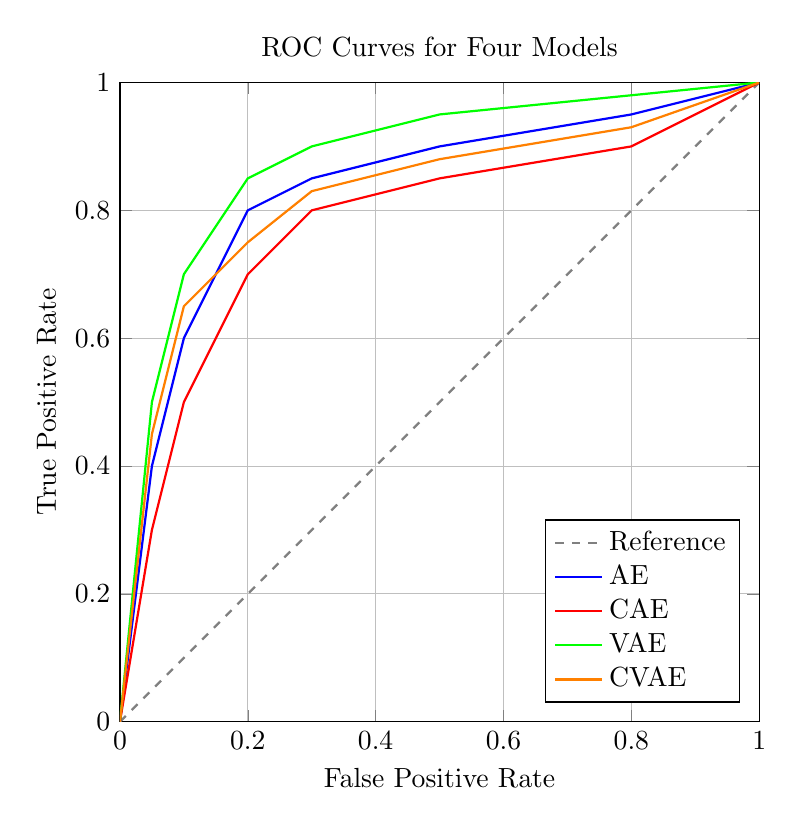
\begin{tikzpicture}
\begin{axis}[
    width=0.8\textwidth,
    height=0.8\textwidth,
    xlabel={False Positive Rate},
    ylabel={True Positive Rate},
    xmin=0, xmax=1,
    ymin=0, ymax=1,
    xtick={0,0.2,0.4,0.6,0.8,1},
    ytick={0,0.2,0.4,0.6,0.8,1},
    legend pos=south east,
    legend cell align={left},
    grid=major,
    title={ROC Curves for Four Models}
]

% Diagonal reference line
\addplot[thick,dashed,gray] coordinates {(0,0) (1,1)};

% ROC curve for Model A
\addplot[thick,blue] coordinates {
    (0,0) (0.05,0.4) (0.1,0.6) (0.2,0.8) (0.3,0.85) (0.5,0.9) (0.8,0.95) (1,1)
};

% ROC curve for Model B
\addplot[thick,red] coordinates {
    (0,0) (0.05,0.3) (0.1,0.5) (0.2,0.7) (0.3,0.8) (0.5,0.85) (0.8,0.9) (1,1)
};

% ROC curve for Model C
\addplot[thick,green] coordinates {
    (0,0) (0.05,0.5) (0.1,0.7) (0.2,0.85) (0.3,0.9) (0.5,0.95) (0.8,0.98) (1,1)
};

% ROC curve for Model D
\addplot[thick,orange] coordinates {
    (0,0) (0.05,0.45) (0.1,0.65) (0.2,0.75) (0.3,0.83) (0.5,0.88) (0.8,0.93) (1,1)
};

\legend{Reference, AE, CAE, VAE, CVAE}

\end{axis}
\end{tikzpicture}
\caption{ROC Curves Comparison for our Autoencoders }
\end{figure}


\begin{figure}[h]
    \centering
    
    % Row 0 (Image Names)
    \begin{subfigure}{0.33\textwidth}
        \centering
        \textbf{Image 1}
    \end{subfigure}%
    \hfill
    \begin{subfigure}{0.33\textwidth}
        \centering
        \textbf{Image 2}
    \end{subfigure}%
    \hfill
    \begin{subfigure}{0.33\textwidth}
        \centering
        \textbf{Image 3}
    \end{subfigure}
    
    \vspace{1em}
    
    % Row 1 (Original)
    \begin{subfigure}{0.33\textwidth}
        \includegraphics[width=\textwidth]{figures/test.png}
        \caption{Original}
    \end{subfigure}%
    \hfill
    \begin{subfigure}{0.33\textwidth}
        \includegraphics[width=\textwidth]{figures/test.png}
        \caption{Original}
    \end{subfigure}%
    \hfill
    \begin{subfigure}{0.33\textwidth}
        \includegraphics[width=\textwidth]{figures/test.png}
        \caption{Original}
    \end{subfigure}
    
    \vspace{1em}
    
    % Row 2 (Model 1)
    \begin{subfigure}{0.33\textwidth}
        \includegraphics[width=\textwidth]{figures/test.png}
        \caption{AE}
    \end{subfigure}%
    \hfill
    \begin{subfigure}{0.33\textwidth}
        \includegraphics[width=\textwidth]{figures/test.png}
        \caption{AE}
    \end{subfigure}%
    \hfill
    \begin{subfigure}{0.33\textwidth}
        \includegraphics[width=\textwidth]{figures/test.png}
        \caption{AE}
    \end{subfigure}
    
    \vspace{1em}
    
    % Row 3 (Model 2)
    \begin{subfigure}{0.33\textwidth}
        \includegraphics[width=\textwidth]{figures/test.png}
        \caption{CAE}
    \end{subfigure}%
    \hfill
    \begin{subfigure}{0.33\textwidth}
        \includegraphics[width=\textwidth]{figures/test.png}
        \caption{CAE}
    \end{subfigure}%
    \hfill
    \begin{subfigure}{0.33\textwidth}
        \includegraphics[width=\textwidth]{figures/test.png}
        \caption{CAE}
    \end{subfigure}
    
    \vspace{1em}
    
    % Row 4 (Model 3)
    \begin{subfigure}{0.33\textwidth}
        \includegraphics[width=\textwidth]{figures/test.png}
        \caption{VAE}
    \end{subfigure}%
    \hfill
    \begin{subfigure}{0.33\textwidth}
        \includegraphics[width=\textwidth]{figures/test.png}
        \caption{VAE}
    \end{subfigure}%
    \hfill
    \begin{subfigure}{0.33\textwidth}
        \includegraphics[width=\textwidth]{figures/test.png}
        \caption{VAE}
    \end{subfigure}
    
    \vspace{1em}
    
    % Row 5 (Model 4)
    \begin{subfigure}{0.33\textwidth}
        \includegraphics[width=\textwidth]{figures/test.png}
        \caption{CVAE}
    \end{subfigure}%
    \hfill
    \begin{subfigure}{0.33\textwidth}
        \includegraphics[width=\textwidth]{figures/test.png}
        \caption{CVAE}
    \end{subfigure}%
    \hfill
    \begin{subfigure}{0.33\textwidth}
        \includegraphics[width=\textwidth]{figures/test.png}
        \caption{CVAE}
    \end{subfigure}
    
    \caption{Comparison of original images and their reconstructions by different autoencodes}
    \label{fig:aereconstruct}
\end{figure}


Apples in my asshole \cite{projthesis}
a \cite{claerbout1991scrutiny}
a \cite{landes1951scrutiny}
a \cite{omar2013machine}
a \cite{wei2022lstmautoencoder}
a \cite{julia}
a \cite{apSensing2019railwaydas}
a \cite{DBLP:journals/corr/SrivastavaMS15}
a \cite{2011ndongsigprocandet}
a \cite{doi:10.1137/141000671}
a \cite{bioengineering10040405}
a \cite{maulik2020recurrent}



\section{Results Setup}

\begin{equation}
    TPR(TruePositiveRate/Recall) = \frac{TP}{TP + FN}
\end{equation}

\begin{equation}
    FPR(FalsePositiveRate/Recall) = \frac{FP}{FP + TN}
\end{equation}

\begin{equation}
    Precision = \frac{TP}{TP + FP}
\end{equation}

\begin{equation}
    F1 - score = 2 x (\frac{Precision \cdot Recall}{Precision + Recall})
\end{equation}

\begin{equation}
    Accuracy = \frac{TP + TN}{TP + TN + FP + FN}
\end{equation}


\begin{tikzpicture}[h]
\centering
  \begin{axis}[ 
    xlabel=$x$,
    ylabel={$relu$},
    xmin=-3, ymax=3,
    ymin=-2, ymax=3,
    grid=both,
  ] 
    \addplot[red, domain=-3:3] {max(0, x)}; 
    
  \end{axis}
\end{tikzpicture}

\begin{table}[h]
\centering
\begin{tabular}{|ll|ll|}
\hline
\multicolumn{2}{|c|}{\multirow{2}{*}{\textbf{Total Population}}} & \multicolumn{2}{c|}{Predictions}      \\ \cline{3-4} 
\multicolumn{2}{|c|}{}                                           & \multicolumn{1}{l|}{Normal} & Anomaly \\ \hline
\multicolumn{1}{|l|}{\multirow{2}{*}{Actual}}      & Normal      & \multicolumn{1}{l|}{TN}     & FP      \\ \cline{2-4} 
\multicolumn{1}{|l|}{}                             & Anomaly     & \multicolumn{1}{l|}{FN}     & TP      \\ \hline
\end{tabular}
\label{tab:confmat}
\caption{Confusion matrix}
\end{table}

\begin{table}[h]
\centering
\begin{tabular}{|l|l|}
\hline
\textbf{Unit} & \textbf{Desc}         \\ \hline
Os            & Ubuntu Linux          \\ \hline
Processor     & Intel i9-9940X @ 4GHz \\ \hline
Ram           & 126GB                 \\ \hline
GPU           & NVIDIA RTX 2080TI     \\ \hline
VRAM          & 11GB                  \\ \hline
Gpu Cores     & 4352                  \\ \hline
Packages      & Flux 2.1., CUDA       \\ \hline
\end{tabular}
\label{tab:specs}
\caption{Specs for our machine running our code}
\end{table}



\subsubsection{Experiment 1: This is how we do it}
\section{Discussion}
\label{chap:discussion}

\section{Modularity in Data Science}

api design for data science has for far long enough been overlooked. Full AI models are regularly being comprised in a single file, with only a argument parser to make sure python can run the script. We instead wanted to seperate between the different aspects of the AI part of the code. The models, engine and hyperparameters can all easily be split into multiple files, but yet this is not common. The advantage we gain by splitting up this module, is easier ways of debugging, as well as to more easily reuse only the sections of the code that we're interested in. Training and Inference are by default split in their own files, since we don't actually want those two run after each other. The training of the neural net should only happen when needed, inference is the mode we'd actually like to test against and return the answers about loss and so on 


\section{Interpretibility}
One major question we wanted to tackle is regarding interpretibility. Is this achieved, or do we still have a long way to go?
\section{Limitations}

Working on Judas with \acrshort{das} data has proven very meaningful. \\\

There are still plenty of undiscovered methods on this kind of data. As mentioned in \cite{MALEKI2021107443}, "Anomaly detection in unlabelled Big Data is difficult and costly". We've seen this occur even after multiple different rounds of resampling, channel decimation, and so on. 
\section{Reflections on Julia}
\label{sec:juliaref}

Intro

Since the very first day of this project, we've been using Julia quite rigorously. Some may argue that C and Python would be more efficient due to their extensive ecosystems and documentations. They are also more or less the \textit{de-facto standard} programming languages for their respective fields, \acrshort{hpc} and \acrshort{ai}. Additionally, members of \acrshort{cgf} are more accustomed to these languages, so why Julia? \\

Besides what's already been mentioned, we wanted to give our thoughts on developing in Julia. Before getting started with Julia as the target language of our program, we made sure it had all the different packages we would need. For \acrshort{ai} and \acrshort{ml} packages, we were pleasantly surprised to find multiple options that all perform well. Bindings to similar packages in Python could also easily be found. We opted for Flux, and with its native integration with CUDA, no extra work had to be done to make use of \acrshort{gpu}s to speed up the computation of our models.

One of the best \\ 
Next to this comes the builtin \texttt{@inbounds} macro, which turns of the boundary checker when accessing memory, speeding up computations in a short matter of time. Not only this, but all the different macros in Julia were pleasant to work with. \texttt{time}, \texttt{btime}, \texttt{profile}, \texttt{cuda}, \texttt{btime}, \texttt{simd} all help imensly when creating programs, without the need for writing loops or custom instructions. Just simply knowing how and where to place macros cleans up the code, and not only increases the developer experience, but also standardizes code between codebases without having to rewrite all from scratch. Just simply running and launcing cudakernels as in \ref{app:jlvsc} shows how easy it is to setup and run CUDA kernels as long as the \texttt{CUDA.jl} package is installed. \\

Version control
A majority of new languages and compilers comes with a version multiplexer, examples being \texttt{rustup}, \texttt{}. These are not built retrospectively, as is the case for \texttt{sdkman} for Java, but before. Managing dependencies and packages, maintaining larger programs and so on becomes a lot easier with both a version multiplexer and a productive package manager. C has never had a standard way of dealing with packages, and this has inspired future languages to extend their ecosystems to include this alongside the compiler and standard library. Python has \texttt{PyPI}, but with many different programs to deal with versioning and packages. Some of these are venv, \texttt{Anaconda} and \texttt{Poetry}. Just simply installing and setting up projects in these languages seem to be harder than it actually have to be, and Julia proves this. \\ 

Enabling multiple processors or threads comes down to simply specifying a flag when running \texttt{-p} or \texttt{-t} respectively. The language has these kinds of computing built into the standard library, no need to install third party dependencies. 

When it comes to AI, Python has stayed supreme as the \textit{de-facto standard} for implementing and testing models. Tensorflow, Pytorch and recently Tinygrad are all highly optimized frameworks for working with ML, with thousands of articles, papers and learning materials written about them. Comparatively, Julias \texttt{Flux.jl} is way younger, but offers in our opinion, easier GPU toggling, model design and overall a smoother experience for . The docs of Flux.jl takes one through the entire codebase, and after reviewing models on \cite{https://github.com/FluxML/model-zoo}, it's easy to figure out how to setup, train and save models.

Julia excels when it comes to scientific computations. Not only does the suppport of unicode symbols make it easier to translate whitepapers to code, but Julias syntax and its compilation makes for an incredible developer experience, as well as increased performance. In the appendix, one can see an example of plotting in Julia, and how intuitive it can be, compared to other languages.






Cons
Although Julia has shown to have many strengths, there is no thing such as a perfect programming language. Julias' main weaknesses besides a far younger ecosystem compared to its alternatives, is its lack of documentation. 

Another potential drawback is the relatively young ecosystem for \acrshort{ai} or \acrshort{ml} programmming that exits compared to Python. As mentioned in \ref{chap:back}, Julia has bindings for Tensorflow, yet still Flux is preferred in most cases. Although it seems to have all functions necessary for computations, some of its functions are not as optimized as they can be. As discussed in \cite{projthesis}, \lstinline|relu| was not optimized until the end of last year. These kinds of optimizations, be it trivial or not, will impact larger programs on a significat level, so we might want to benchmark certain functions to see if they may be optimized futher. However, this is also a great aspect of Julia. Since Flux is natively written in Julia, replacing old functions with more optimized or type specific functions seem to  


Conclusions on personal use 


\chapter{Conclusion}
\label{chap:conclusion}

dkl

\section{Further work}
\label{conc:further}

While our work has addressed several key challenges, both Judas and TinyDAS are in their first iterations. Further research and development can address the current limitations discussed in this thesis.

\subsection{Judas and \acrshort{das} processing}

While Judas serves the task of loading and processing \acrshort{das} data, the following list provides an overview of further advancements that can enhance its computational effectiveness, specifically targeting file loading:

\begin{itemize}
    \item Design and implement a more course-grained approach to our current solutions for finding and loading \acrshort{das} files. 
    \item Designing a parallel version of the column-wise cumulative sum function, potentially using algorithms like parallel prefix sum \cite{harris2007parallel}, where \acrshort{gpu} acceleration could be introduced. 
    \item Implementing a more flexible metadata handling system to accommodate datasets from other sources besides BANENOR.
    \item Implementing more advanced denoising and signal processing techniques, potentially utilizing denoising autoencoders \cite{eage:/content/journals/10.1111/1365-2478.13355}.
\end{itemize}

\subsection{TinyDAS and Autoencoder-based Anomaly Detection}

As discussed in Section \ref{disc:tinydas}, we have succeeded in many of our goals with TinyDAS. However, as the poor results from the variational autoencoders show, there is still much room left for tuning current models. The following list presents multiple avenues for further development and research:

\begin{itemize}
    \item Expand support for more different architecture and compare simpler models with hybrid models that combine both the temporal and spatial aspects of \acrshort{das} signals, such as CNN-LSTM architectures, or even transformer-based ones, to capture finer details.
    \item  Half-precision training has been a heavy area of attention. For now, TinyDAS supports half-precision training, inference, loss-scaling, and gradient clipping. Further improving on these to ensure gradients are within range is an important aspect of reducing runtime and memory consumption. Comparing this approach to mixed-precision could prove beneficial.
    \item Expanding support for other \acrshort{das} datasets, both from PubDAS and other public sources. This could be achieved through a more customizable format of our DataLoader class. Furthermore, implementing functionality for downloading \acrshort{das} datasets directly from the internet would lower the user entry barrier.
    \item Implement support for reading real-time datastreams, to further analyze how different models perform in real-world scenarios
\end{itemize}

\subsection{Final Remarks}

We want to thank \acrfull{cgf} for providing data and computational resources. We hope both these programs can help all their current and future members further the field of \acrshort{das} research.


\chapter*{\bibname}
\printbibliography[heading=none]

\appendix
\chapter{Example of Scientific Computation in Julia}
\label{app:jlscicomp}

\begin{figure}[h]
    \centering
    \lstinputlisting{"code/waves.jl"}
    \caption{Caption}
    \label{fig:enter-label}
\end{figure}

\section{Subtyping in Julia}
\label{app:subtyping}

\begin{figure}[h]
    \centering
    \lstinputlisting{"code/subtyping.jl"}
    \caption{Example with subtyping in Julia. Here we make use of multiple dispatch as well to create }
    \label{fig:subtyping}
\end{figure}
\chapter{PubDAS Foresee Data Preprocessing}
\label{app:pubdas}

\lstset{style=pstyle}
\lstinputlisting[language=Python, caption=Preprocessing of the FORESEE dataset from TDMS to HDF5]{code/pubdas.py}
\chapter{CUDA in Julia vs C}
\label{app:jlscicomp}

\begin{figure}[h]
    \centering
    \lstinputlisting{"code/jlcuda.jl"}
    \caption{Launching CUDA kernel in Julia. This can be run directly with the Julia compiler}
    \label{fig:jlcuda}
\end{figure}
 
\begin{figure}[h]
    \centering
    \lstinputlisting{"code/ccuda.c"}
    \caption{Launching CUDA kernel in C. This code can't be compiled without the NVIDIA compiler, and needs to be stored as a .cu file}
    \label{fig:ccuda}
\end{figure}
\chapter{MNIST Classifier in Julia}
\label{app:juliamnist}

\begin{figure}[h]
    \centering
    \lstinputlisting{code/mnist.jl}
    \caption{Mnist in Julia}
    \label{fig:juliamnist}
\end{figure}
\chapter{Hyperparameters and Configurations in TinyDAS}
\label{app:configs}

\section{Hyperparameters}

\begin{figure}[h]
  \begin{subfigure}[t]{.45\textwidth}
    \centering
    \lstinputlisting{code/configs/ae.yaml}
    \caption{AE}
  \end{subfigure}
  \hfill
  \begin{subfigure}[t]{.45\textwidth}
    \centering
    \lstinputlisting{code/configs/cnnae.yaml}
    \caption{CNN AE}
  \end{subfigure}

  \medskip

  \begin{subfigure}[t]{.45\textwidth}
    \centering
    \lstinputlisting{code/configs/vae.yaml}
    \caption{VAE}
  \end{subfigure}
  \hfill
  \begin{subfigure}[t]{.45\textwidth}
    \centering
    \lstinputlisting{code/configs/betavae.yaml}
    \caption{Beta VAE}
  \end{subfigure}
    \caption{Hyperparameters for all models}
\end{figure}

\section{Configurations}

\begin{figure}[h]
    \centering
    \lstinputlisting[language=sh, caption=Slurm script example]{code/configs/ae.sh}
    \label{fig:slurmconf}
\end{figure}


\chapter{Judas}
\label{app:judas}


\section{Packages Used}
\label{app:jupacks}

\begin{table}[!h]
\centering
\caption{Packages used in Judas}
\label{tab:judas-packages}
\small
\begin{tabular}{>{\raggedright\arraybackslash}p{0.25\textwidth}>{\raggedright\arraybackslash}p{0.65\textwidth}}
\toprule
\textbf{Package Name} & \textbf{Description} \\
\midrule
%\rowcolor{gray!10} Flux & AI library \\
CUDA & NVIDIA CUDA programming \\
\rowcolor{gray!10} DSP & Digital Signal Processing \\
DataFrames & Working with Dataframes \\
\rowcolor{gray!10} JLD2 & Saving and loading of models \\
HDF5 & HDF5 wrapper for Julia \\
\rowcolor{gray!10} LinearAlgebra & Linear Algebra package \\
Statistics & Distributions and common functions for statistics\\
\rowcolor{gray!10} Mmap & Memory mapped I/O for working with large arrays \\
Distributed & Parallel computing in Julia \\
\rowcolor{gray!10} FFTW & FFTW wrapper for Julia \\
Dates & Datetime library \\
\rowcolor{gray!10} Plots & Plotting utilities \\
Colors & Extra colorschemes for plots \\
\rowcolor{gray!10} BenchmarkTools & Benchmark tools and utilities \\
SymPy & Julia wrapper for working with symbolic notation \\
\bottomrule
\end{tabular}
\end{table}

\section{Load DAS Files function}
\label{app:loaddas}
\lstinputlisting[label={code:loaddas},caption=Load DAS Files, language=Julia]{code/loaddas.jl}
\chapter{Packages Used}
\label{app:packages}

\section{Judas}
\label{app:jupacks}

\begin{table}[h]
\begin{tabular}{|l|l|}
\hline
\textbf{Name}  & \textbf{Description}                             \\ \hline
Flux           & AI library                                       \\ \hline
CUDA           & NVIDIA CUDA programming                          \\ \hline
DSP            & Digital Signal Processing                        \\ \hline
DataFrames     & Working with Dataframes                          \\ \hline
JLD2           & Saving and loading of models                     \\ \hline
HDF5           & HDF5 wrapper for Julia                           \\ \hline
LinearAlgebra  & Linear Algebra package                           \\ \hline
Statistics     & Distrbiutions and common functions               \\ \hline
Mmap           & Memory mapped I/O for working with large arrrays \\ \hline
Distributed    & Parallel computing in Julia                      \\ \hline
FFTW           & FFTW wrapper for Julia                           \\ \hline
Dates          & Datetime library                                 \\ \hline
Plots          & Plotting utilities                               \\ \hline
Colors         & Extra colorschemes for plots                     \\ \hline
BenchmarkTools & Benchmark tools and utilities                    \\ \hline
SymPy          & Julia wrapper for working with symbolic notation \\ \hline
EvalMetrics    & PR plot and AUC                                  \\ \hline
MLBase         & Common ML utilities                              \\ \hline
cuDNN          & NVIDIA cuDNN wrapper for Julia                   \\ \hline
\end{tabular}
\end{table}


\section{TinyDAS}
\label{app:tinypacks}

\begin{table}[h]
\centering
\begin{tabular}{|l|l|}
\hline
\textbf{Name}  & \textbf{Description}                             \\ \hline
tinygrad          & AI library                                       \\ \hline
h5py           & NVIDIA CUDA programming                          \\ \hline
pyyaml            & Digital Signal Processing                        \\ \hline
numpy          & Numeric programming \\ \hline
\end{tabular}
\end{table}
\chapter{Trainmap BaneNOR}
\label{app:jlscicomp}

\begin{figure}[h]
    \centering
    \includegraphics[scale=0.5]{figures/togkart.png}
    \caption{Map over train route from Trondheim to Storen}
    \label{fig:trainmap}
\end{figure}

\end{document}
